\subsection{Impact: Process Count}\label{sec:dspmv-process}

\begin{figure*}\begin{centering}
		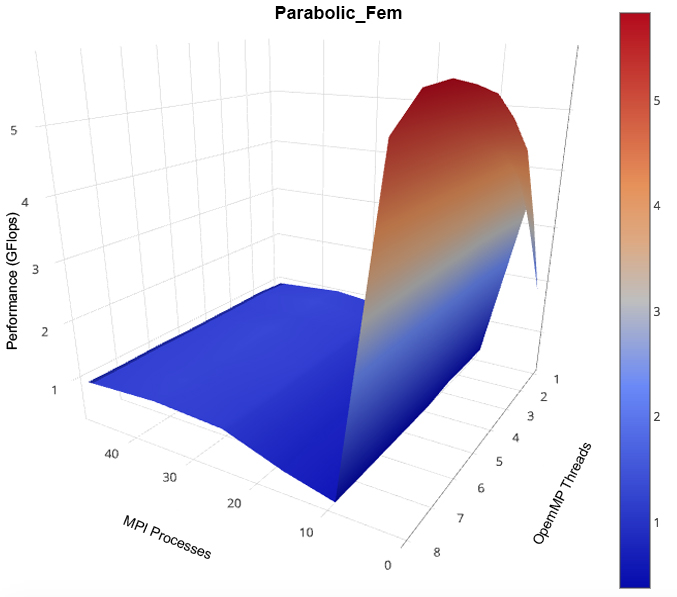
\includegraphics[scale=0.25]{figures/parabolicFem_surface.jpg}
		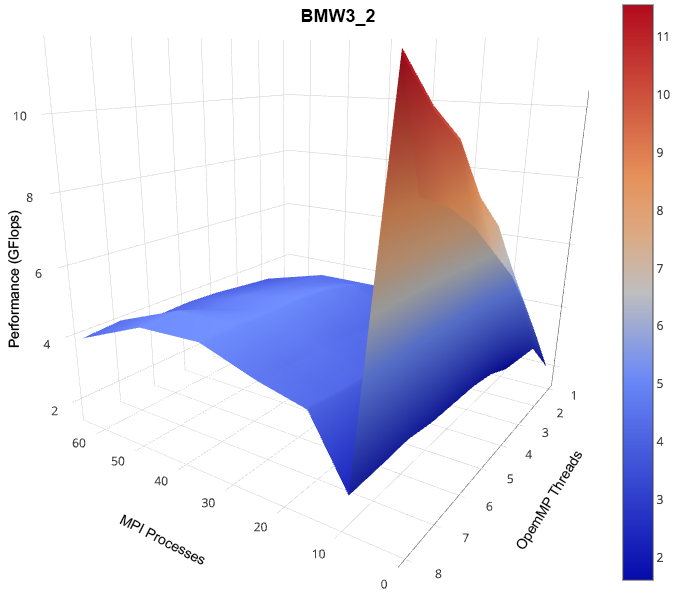
\includegraphics[scale=0.25]{figures/bmw3_2_surface.jpg}
		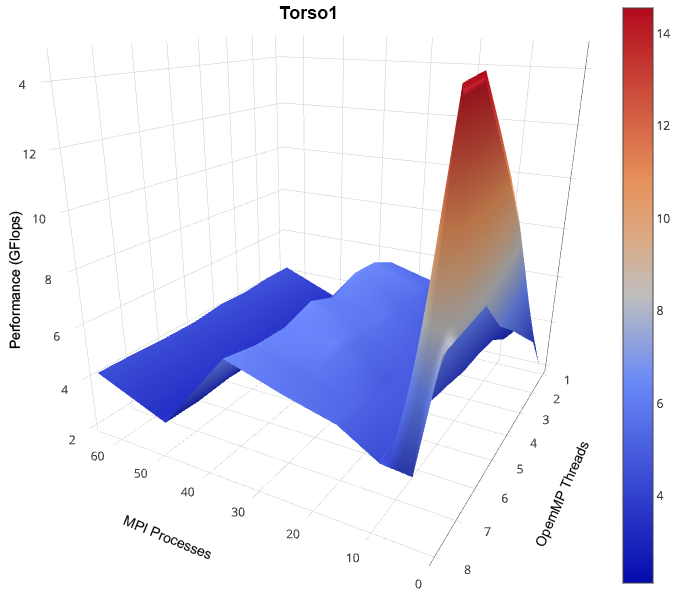
\includegraphics[scale=0.25]{figures/torso1_surface.jpg}
		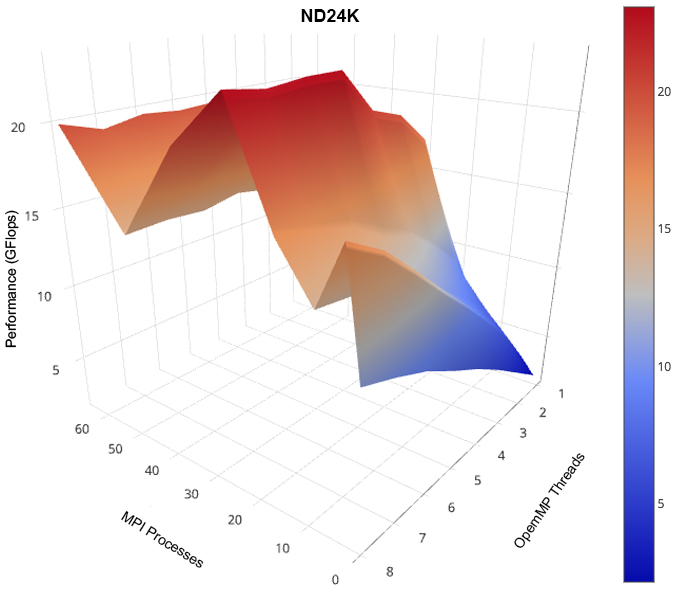
\includegraphics[scale=0.25]{figures/nd24k_surface.jpg}
		\caption{Hybrid SpMV Performance for Matrices with varying Sparsity}
		\label{fig:spmv-matrix-surfaces}
\end{centering}\end{figure*}

\begin{figure*}\begin{centering}
		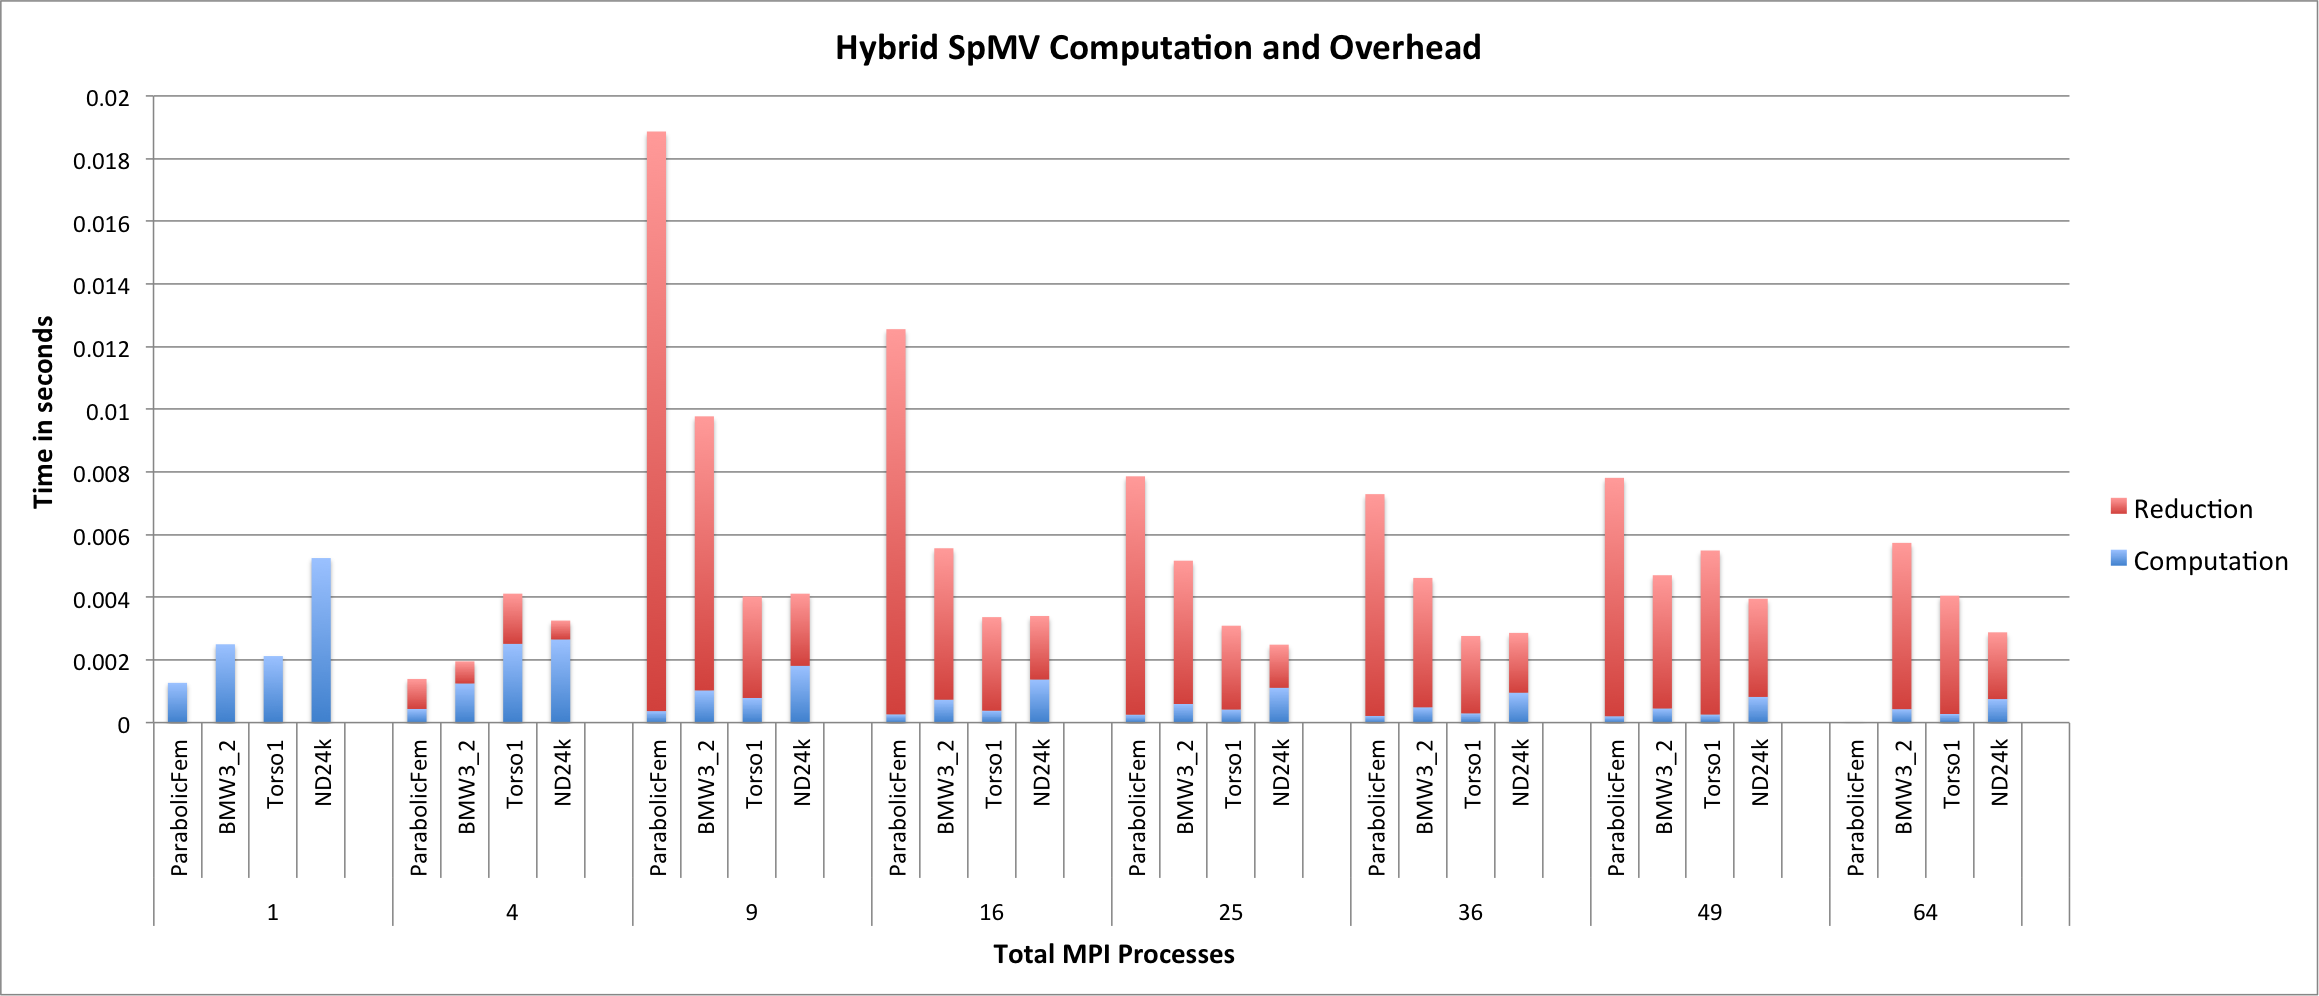
\includegraphics[scale=0.35]{figures/stackedbar_overhead.png}
		\caption{Computational Time and Reduce + Barrier Overhead}
		\label{fig:spmv-comp-and-reduction}
\end{centering}\end{figure*}

Increasing the number of processes eventually requires the use of additional nodes, thus introducing communication overhead.
We examined the performance impact of scaling up $p$ such that a node had between 1 and 16 processes. Subsequently we scaled thread count so that all available processing hardware on a node was used during the study. The performance characteristics for 2 MPI processes per node (where applicable) with varying total process count and threads per process are visible in Fig. \ref{fig:spmv-matrix-surfaces}. 

For all but the least sparse matrix performance accelerates quickly until 9-16 processes, followed by a sharp decline as overhead from the non-logarithmic \emph{MPI\_Reduce} outpaced the benefit of additional processes. These results agree with the analytical model from \ref{sec:spmv-analytic} where in such a decline is exhibited in Fig. \ref{fig:spmv-analytic-model}(a) for the Non-Overlapping case. Due to an inability to increase $p$ beyond 64 total processes ($8$x$8$ process matrix), our results did not indicate if nd24k would experience similar behavior, however, due to the impact sparsity has on performance at scale, it is likely that the trend exhibited in \ref{fig:spmv-analytic-model}(a) would hold true. 
